\chapter{Футбол}

Една от любимите игри за децата е футболът. Целта на тази игра е играчът да вкара максимално много гола. Ако пропусне - играта приключва.

\begin{figure}[H]
  \centering
  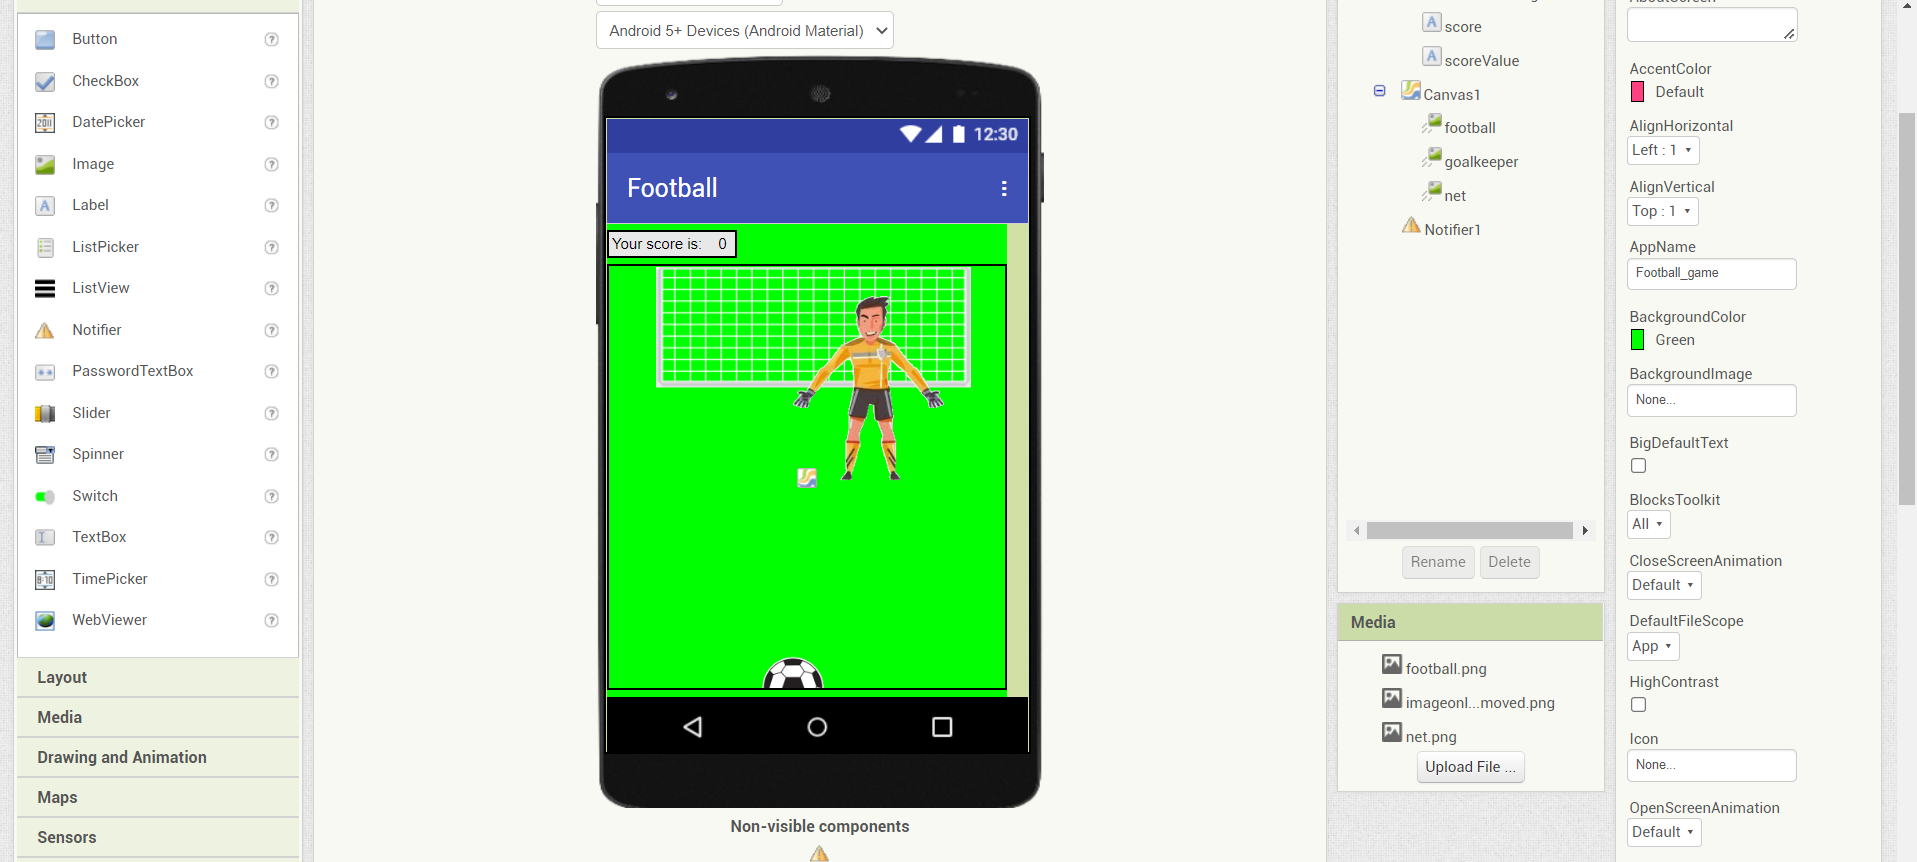
\includegraphics[width=1.0\linewidth,height=0.5\linewidth]{fig110001.png}
  \caption{Футбол}
\label{fig110001}
\end{figure}

\section{Създаване на дизайн на играта}
Първата стъпка от създаването на тази игра е добавяне на всички компоненти, които ще бъдат програмирани. Цветът на игрището трябва да бъде зелен, за това трябва да се промени стойността на свойството BackgroundColor да бъде зелен.

\begin{figure}[H]
  \centering
  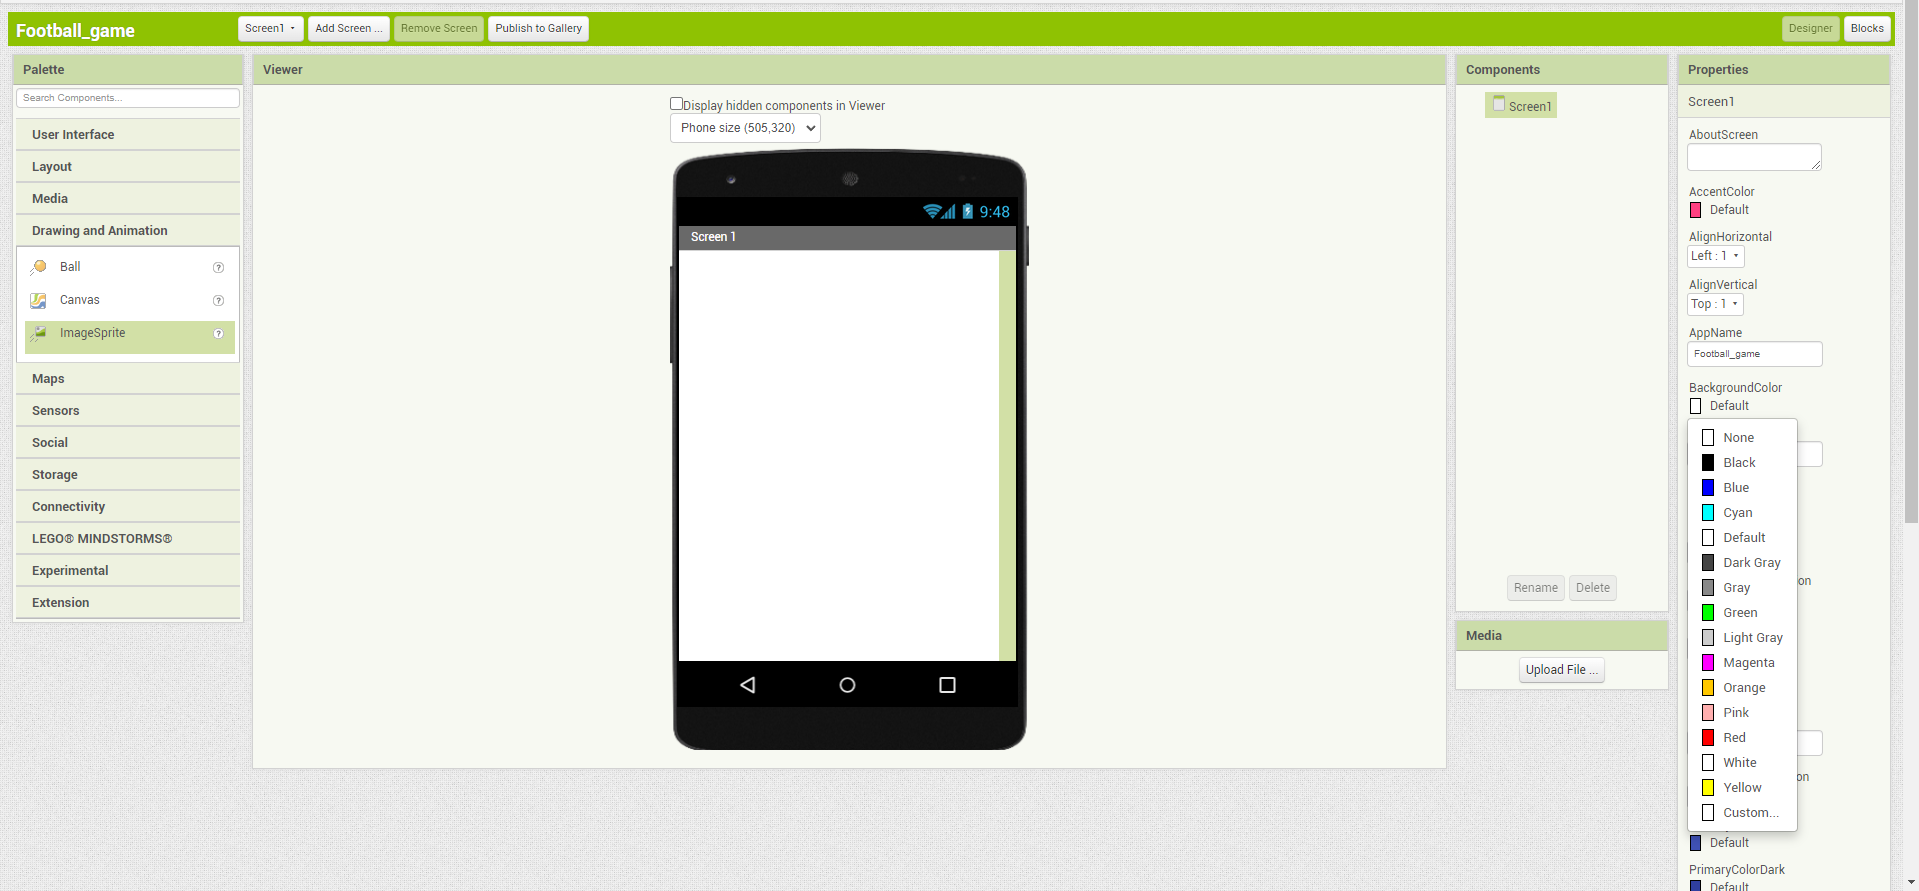
\includegraphics[width=1.0\linewidth,height=0.5\linewidth]{fig110002.png}
  \caption{Промяна на цвета на фона}
\label{fig110002}
\end{figure}

Една от най- важните задачи при програмирането на мобилни приложения е техния интерфейс. За да се направи по- атрактивна тази игра може да се смени стойността на свойството Theme да бъде Device Default, а името на свойството Title да бъде Footbal.

\begin{figure}[H]
  \centering
  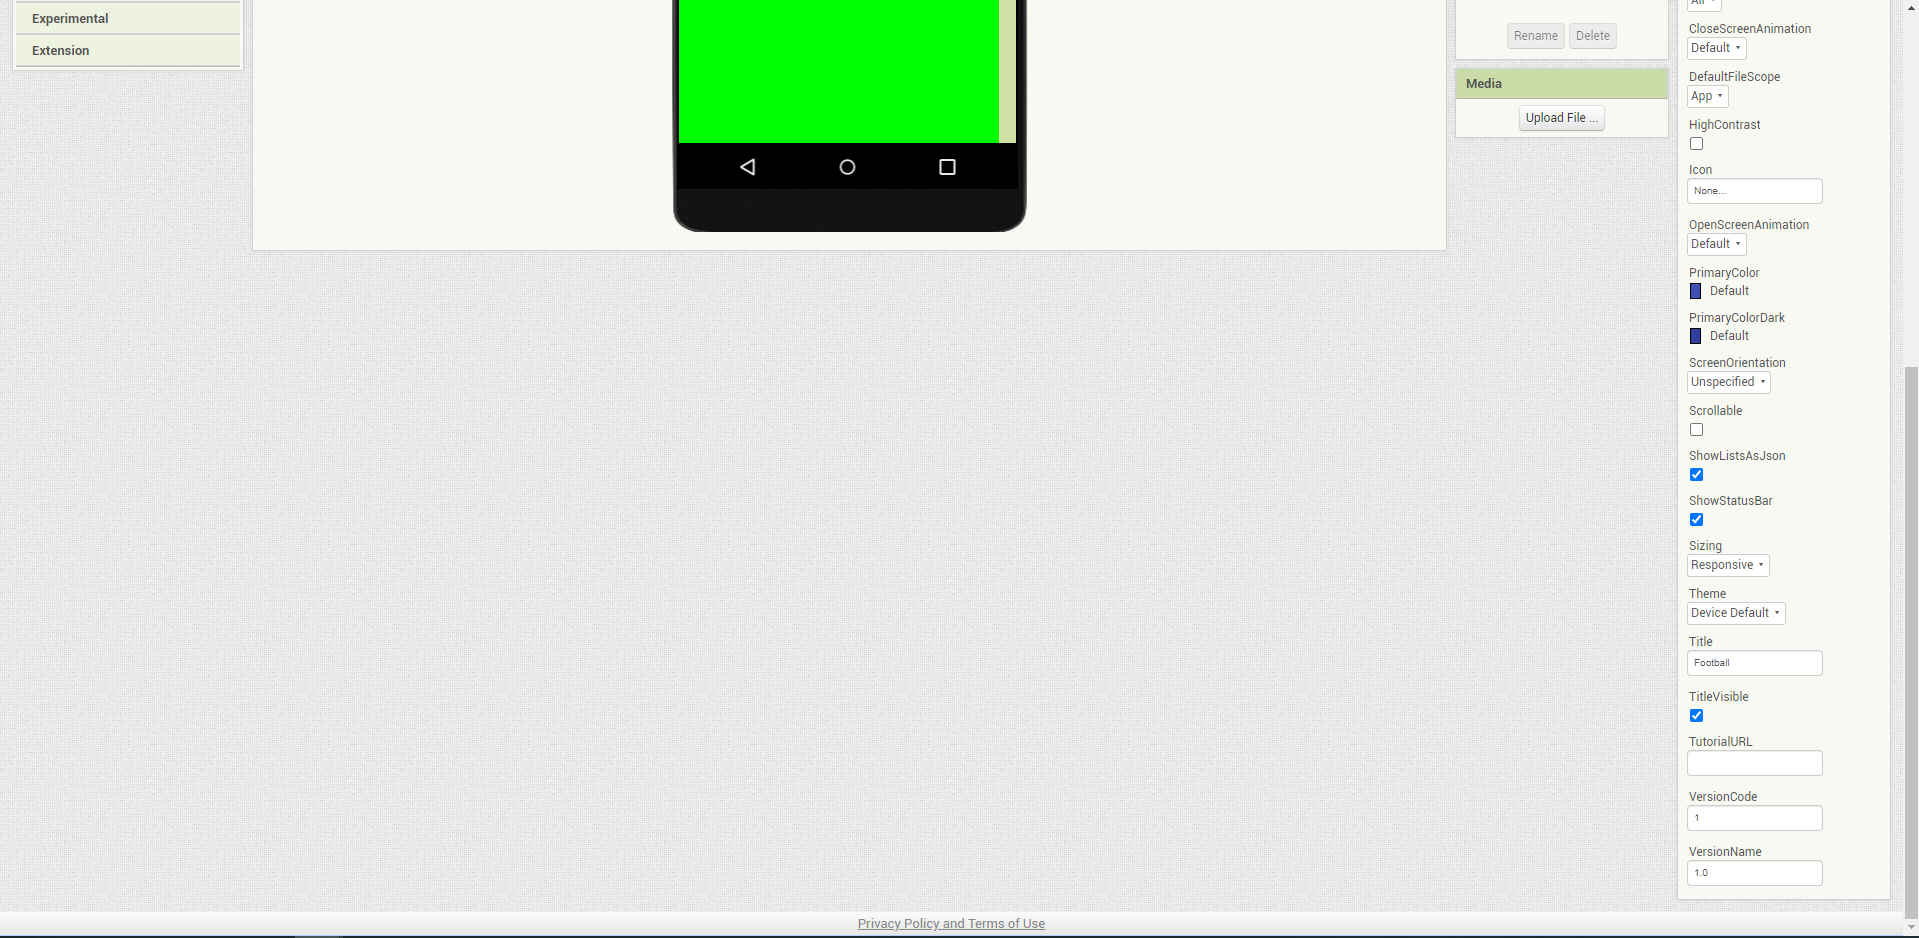
\includegraphics[width=1.0\linewidth,height=0.5\linewidth]{fig110003.png}
  \caption{Промяна на темата}
\label{fig110003}
\end{figure}

За да може играчът да изстрелва топката, когато докосне екрана на телефона си, а също и вратаря да се движи по екрана, трябва да се добави елементът Canvas. Ширината и височината му трябва да бъде същата каквато е на екрана на телефона. За да се направи това се задават стойности на свойството Height да бъде Fill parent... Същата е и стойността на свойството Width. Този елемент трябва да се слее с цвета на фона. За тази цел трябва да се промени стойността на свойството BackgroundColor.

\begin{figure}[H]
  \centering
  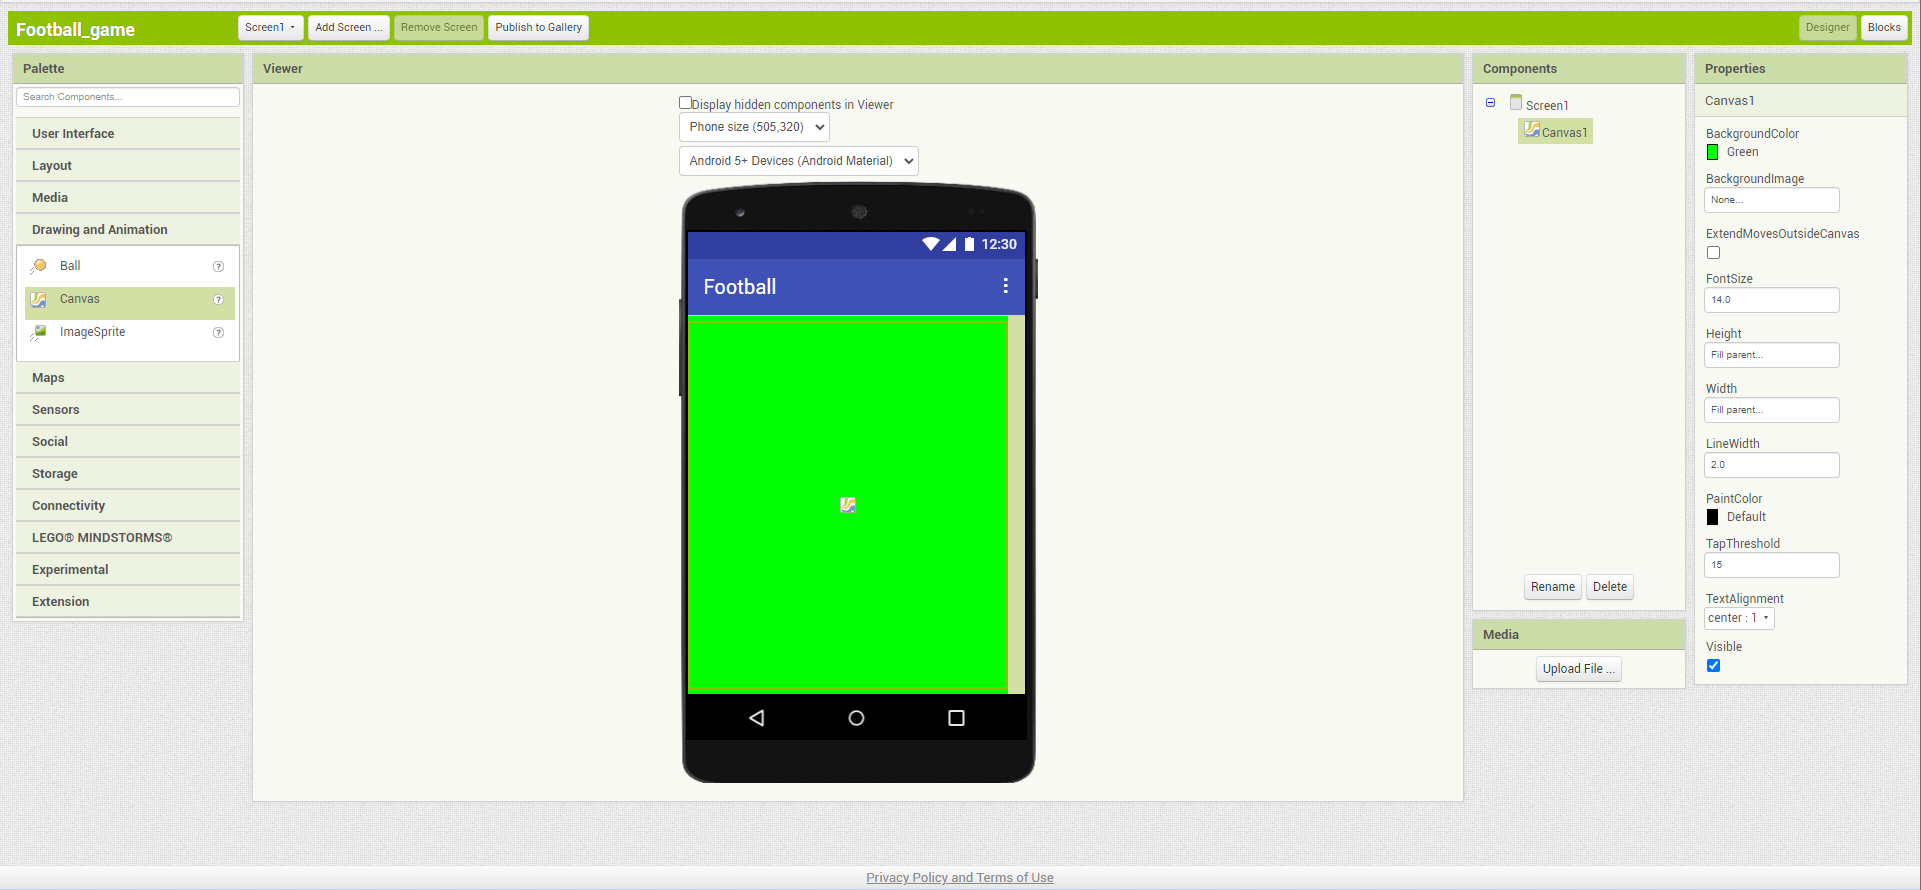
\includegraphics[width=1.0\linewidth,height=0.5\linewidth]{fig110004.png}
  \caption{Елементът Canvas}
\label{fig110004}
\end{figure}

Следва да се добавят три елемента ImageSprite съответно за мрежата, вратаря и топката. Може да се преименуват, за да бъде ясно кой елемент за какво е. За изображенията на тези елементи може да се използват картинки, които се разпространяват със свободен лиценз за не търговска употреба.

\begin{figure}[H]
  \centering
  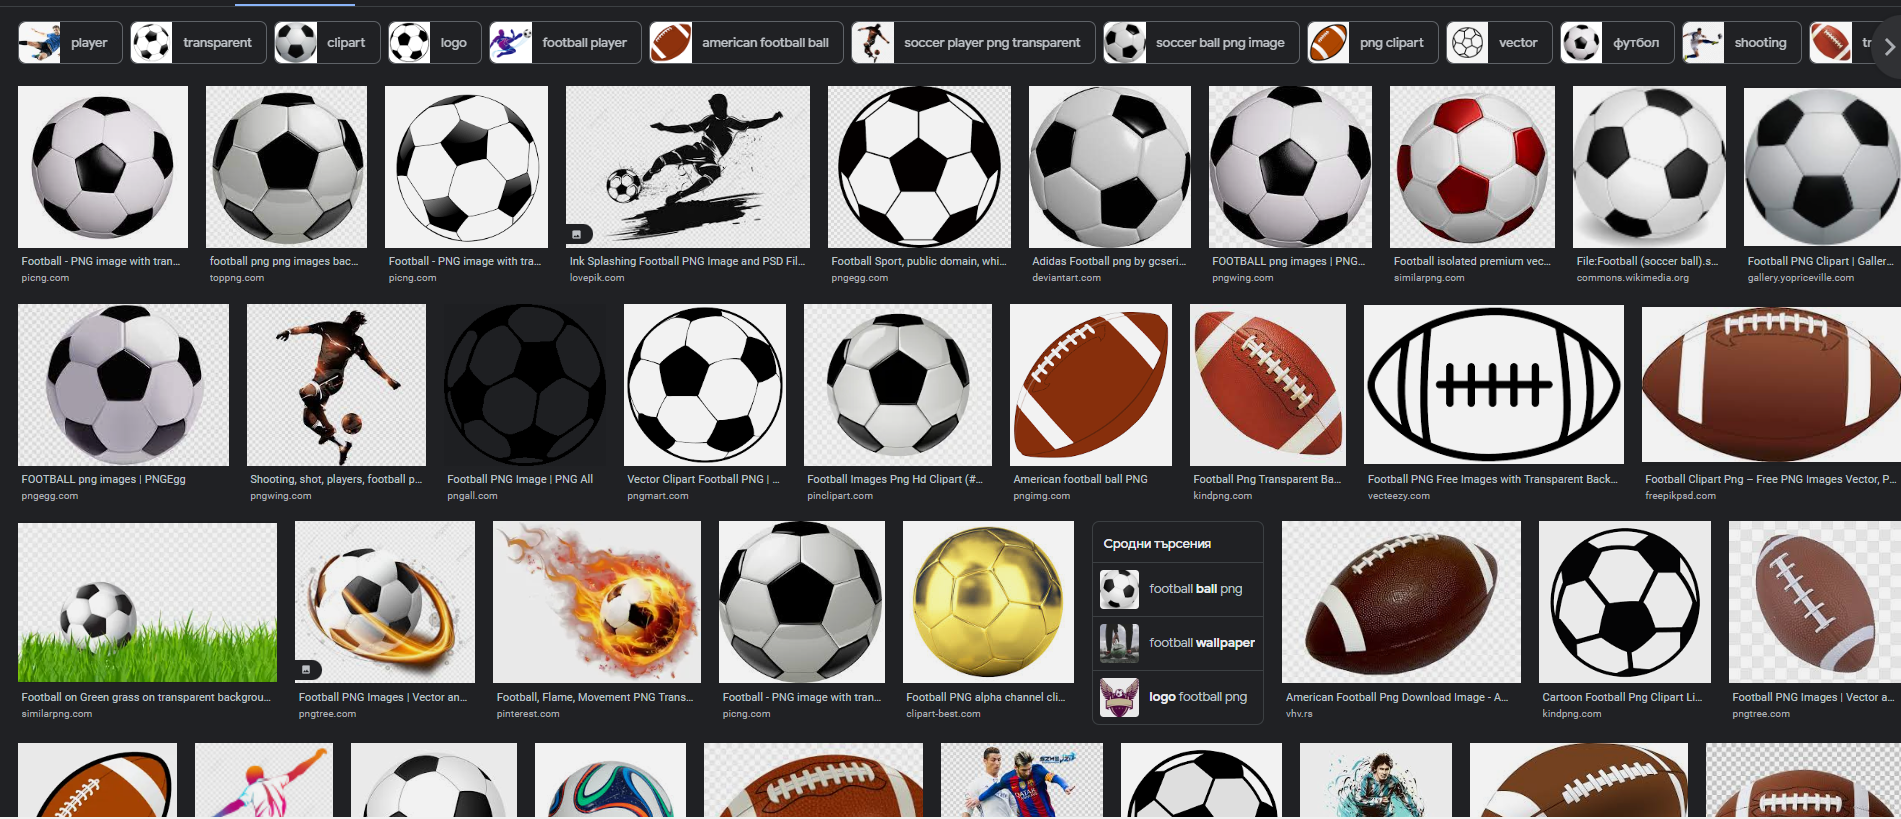
\includegraphics[width=1.0\linewidth,height=0.5\linewidth]{fig110005.png}
  \caption{Изображение на футболна топка}
\label{fig110005}
\end{figure}

След като изображенията са налични трябва да се поставят на съответните ImageSprite елементи и да се променят свойствата за височина, ширина и позиция. Това означава, че трябва да се оразмерят спрямо екрана на телефона. Крайният резултат трябва да изглежда така:

\begin{figure}[H]
  \centering
  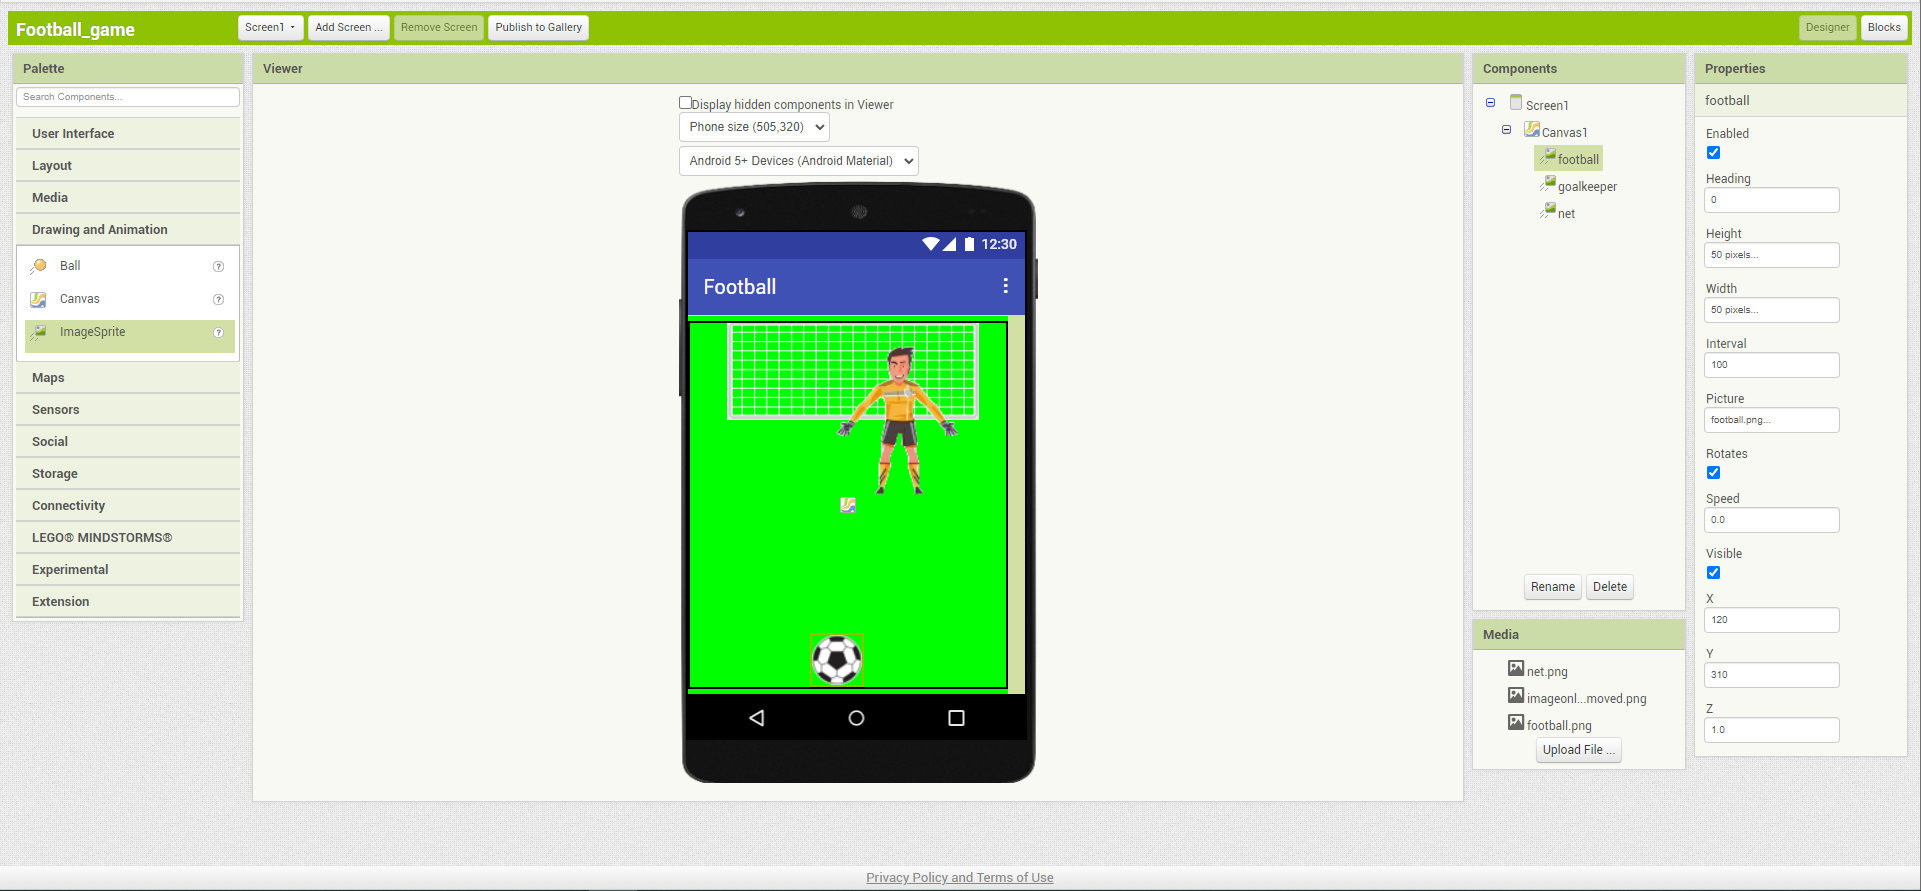
\includegraphics[width=1.0\linewidth,height=0.5\linewidth]{fig110006.png}
  \caption{Дизайн на играта}
\label{fig110006}
\end{figure}

Освен тези елементи, трябва да се добави и място, където ще се изписва резултатът. От групата с елементи Layout трябва да бъде добавен елментът HorizontalArrangement, за да може вътре в него да се поставят два елемента Label. Единият ще е за съобщението за резултатът, а вторият ще е за стойността на резултатът. Това означава, че стойността на свойството за първия етикет ще е "Your score is: ", а за втория - "0". Добра практика е да се преименуват елементите, за да може по- лесно да се програмират. В по- късен етап от играта ще има нужда и от елемента "Notifier". Той е от групата на скритите елементи.

\begin{figure}[H]
  \centering
  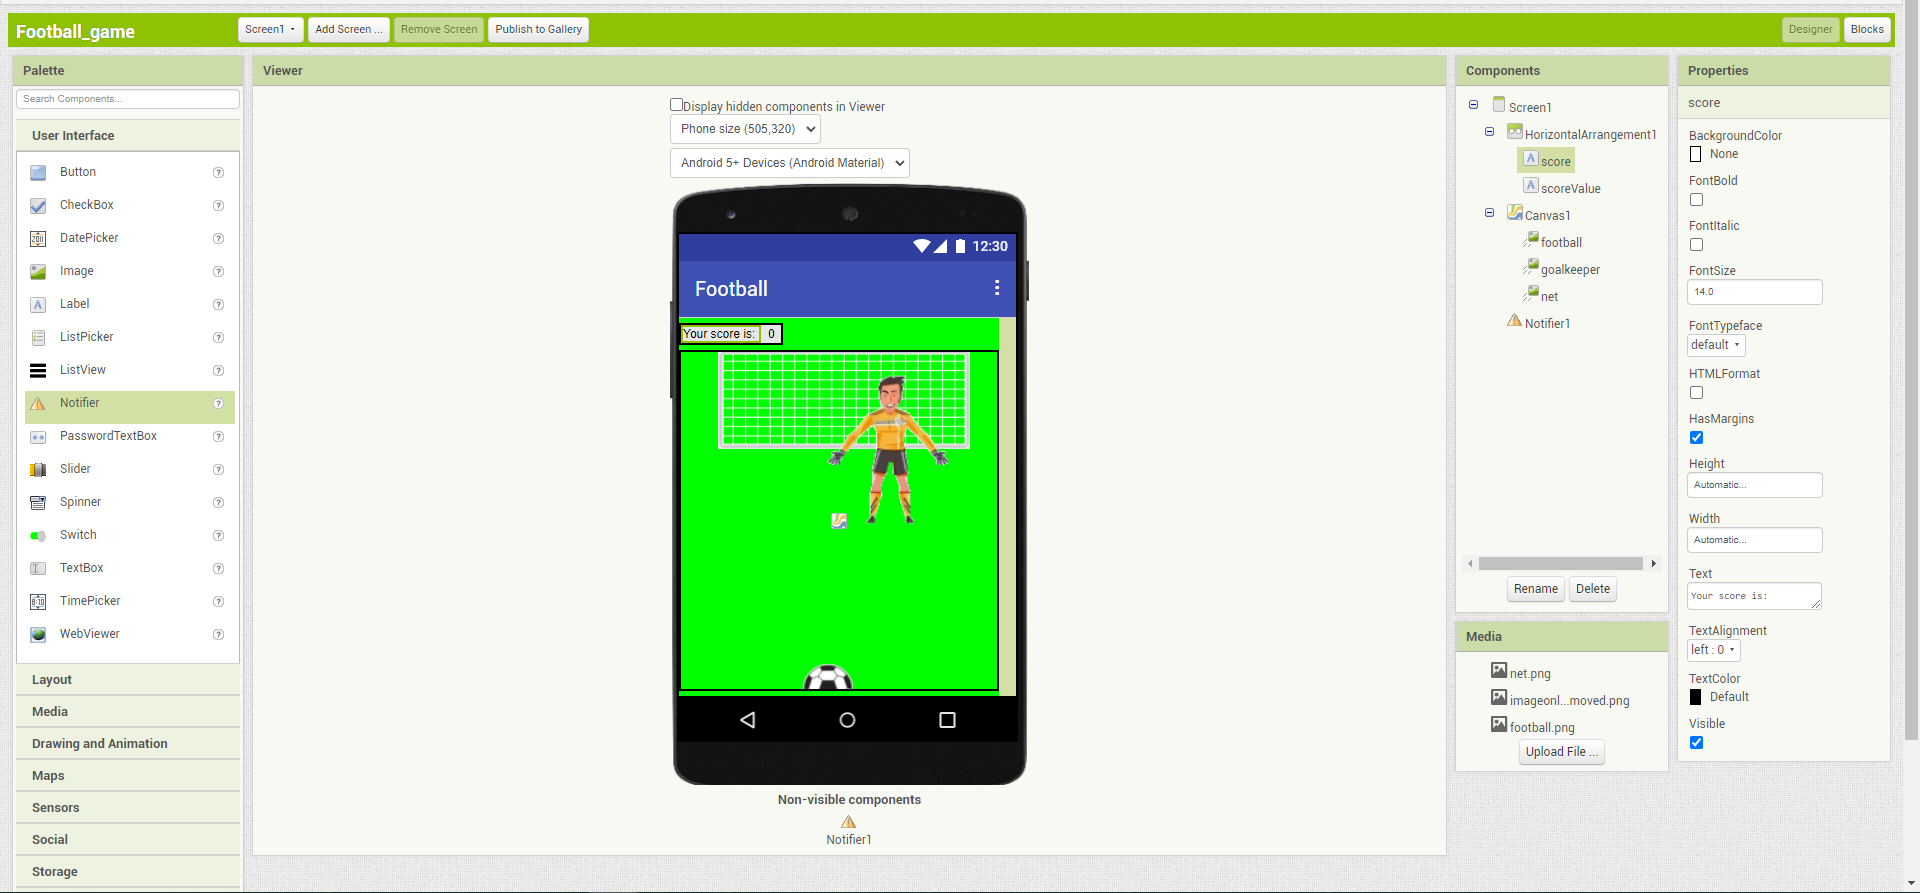
\includegraphics[width=1.0\linewidth,height=0.5\linewidth]{fig110007.png}
  \caption{Всички елементи на играта}
\label{fig110007}
\end{figure}

\section{Програмиране}
Следва да се добавят и необходимите инструкции към елементите, които са добавени за играта. За тази цел трябва да се премине към другия изглед, който е за добавяне на инструкциите.

Първвите инструкции ще са за вратаря. Той ще се движи в ляво и дясно. Неговата цел е да пази вратата от това да се вкара гол. Когато играта започне, вратаря трябва да започне да се движи. Това означава, че трябва да се добави инструкцията when Screen1.Initialize, която се намира в елемента Screen1. Вътре в това събитие трябва да се добавят две инструкции, които се намират в елемента goalkeepr. Едната инструкция е да се зададе стойност на свойството Interval, което определя на колко милисекунди ще се променя позицията на този герой. Втората инструкция задава стойност на свойството Speed, което отговря за движението на героя.

Още едно събитие трябва да се добави - when goalkeeper.EdgeReached. Инструкциите от това събитие ще се изпълнят, тогава, когато вратаря докосне ръба на екрана. Когато това стане се извиква инструкцията goalkeeper.Bounce edge, а стойността която се поставя е get edge.

\begin{figure}[H]
  \centering
  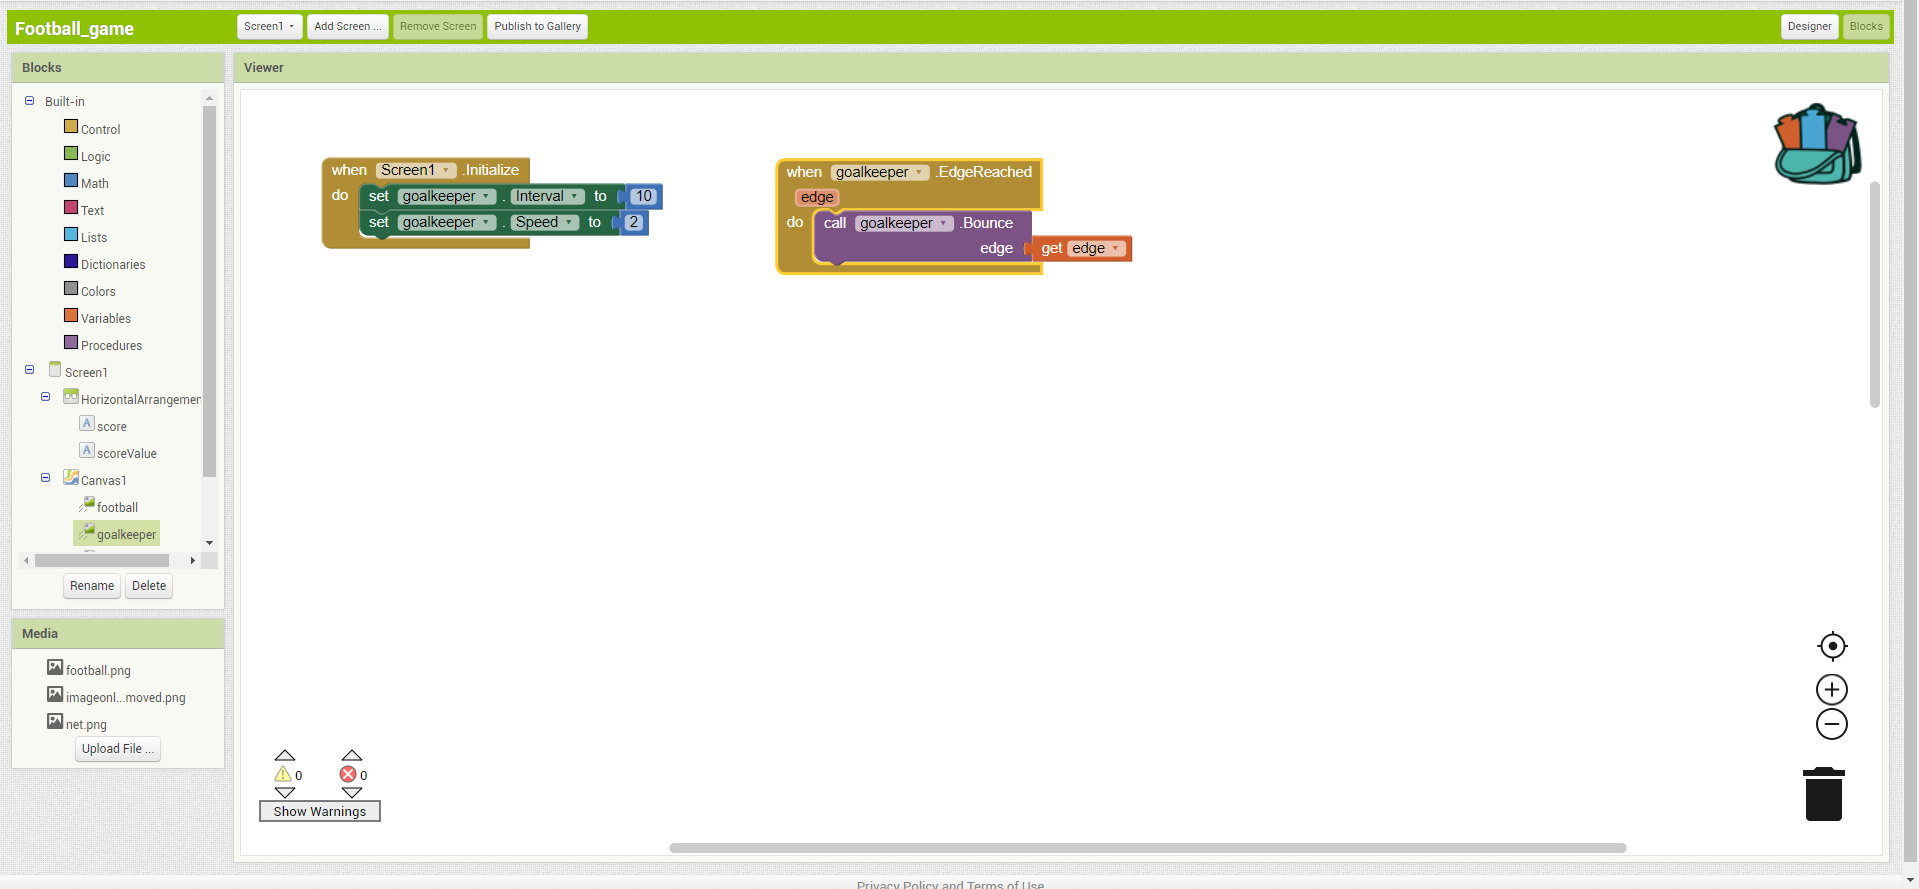
\includegraphics[width=1.0\linewidth,height=0.5\linewidth]{fig110008.png}
  \caption{Движение на вратаря}
\label{fig110008}
\end{figure}

Когато се стартира играта се забелязва, че вратаря се завърта с надолу главата. Това може да се промени, като се размаркира свойството Rotates.

\begin{figure}[H]
  \centering
  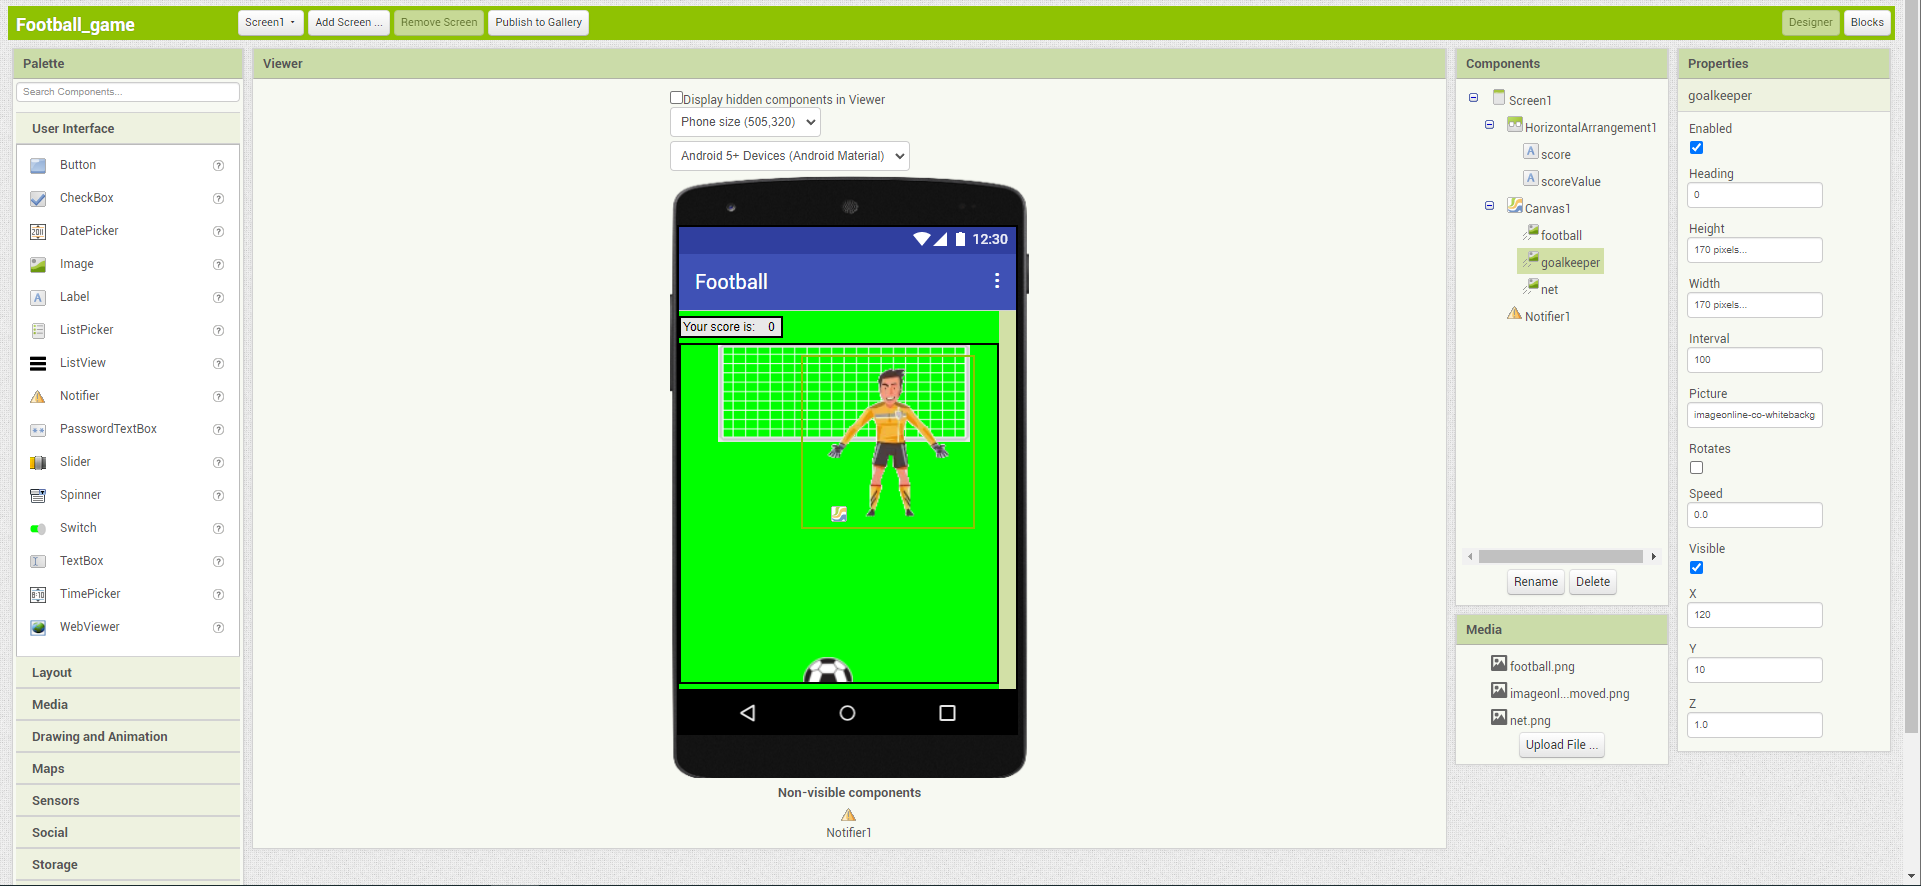
\includegraphics[width=1.0\linewidth,height=0.5\linewidth]{fig110009.png}
  \caption{Спиране на въртенето на вратаря}
\label{fig110009}
\end{figure}

Следва да се добавят инструкции за това, когато играчът плъзне топката, тя да се движи. Първо трябва да се добави събитието when football.Flug. Аналогично на вратаря трябва да се зададат стойности за Interval и Speed. Стойността на свойството Interval трябва да бъде 10, а тази за Speed 20. Освен движението трябва да се зададе и ъгълът, в който ще се движи топката. За тази цел трябва да се зададе стойност за свойството Heading, която идва от събитието - get heading.

\begin{figure}[H]
  \centering
  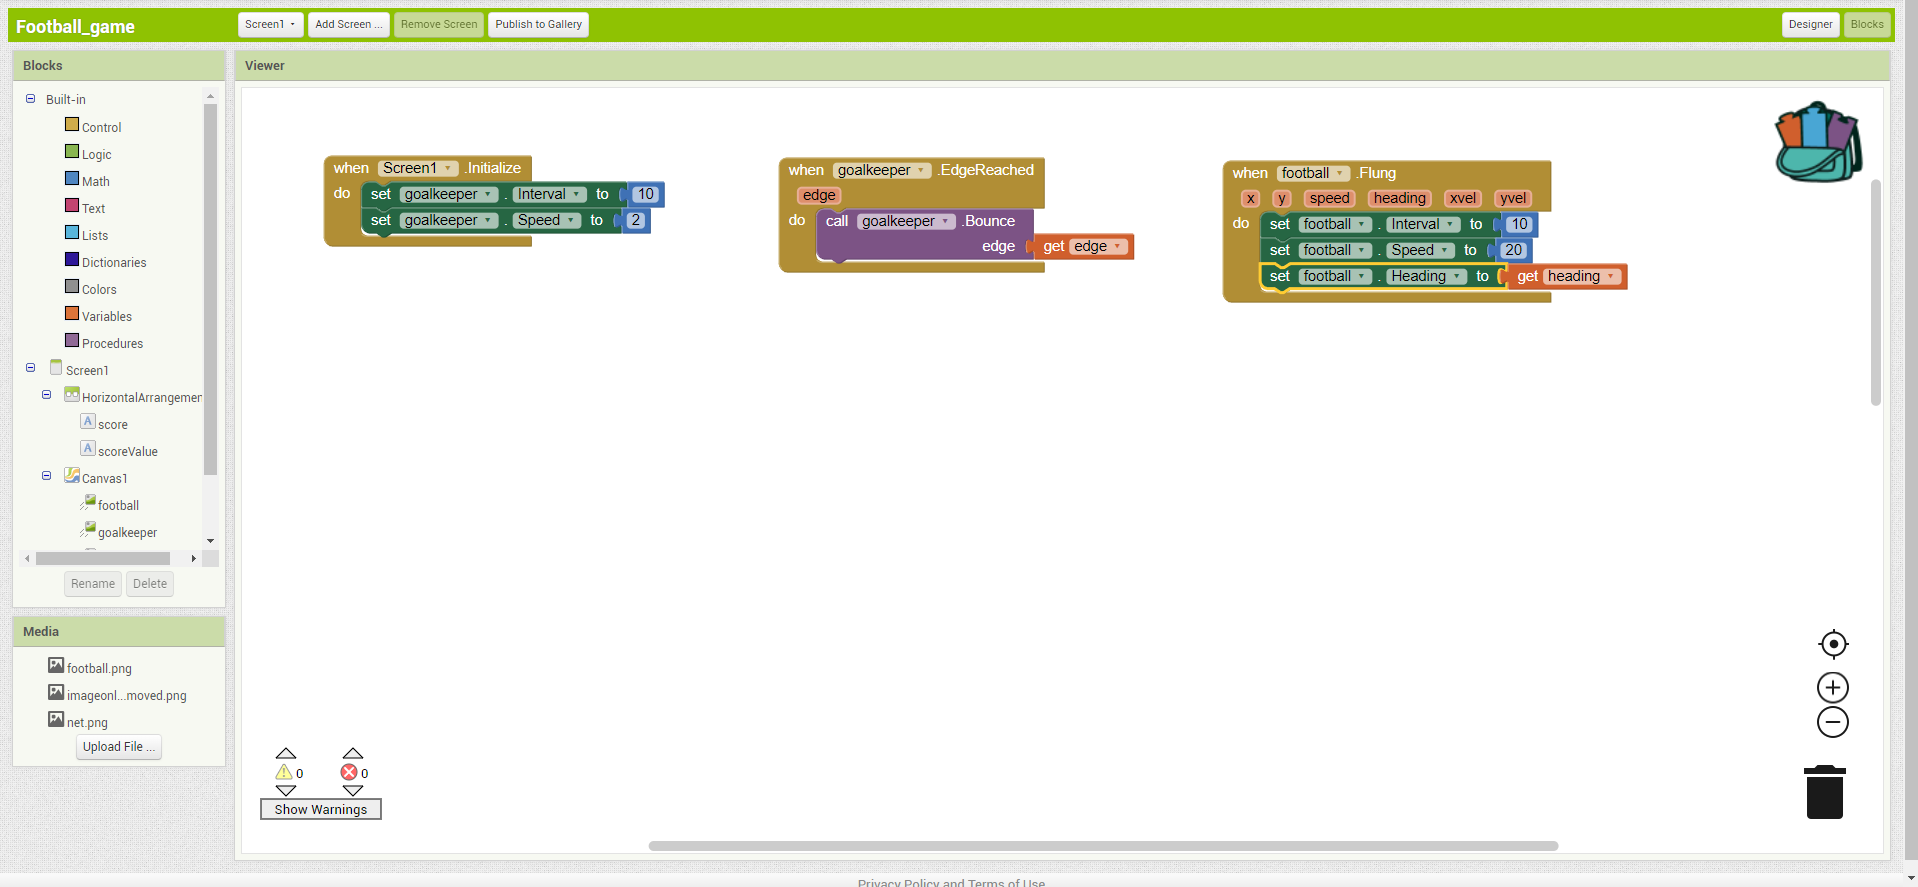
\includegraphics[width=1.0\linewidth,height=0.5\linewidth]{fig110010.png}
  \caption{Движение на топката}
\label{fig110010}
\end{figure}

В последната фаза на играта трябва да се програмира какво се случва когато топката докосне мрежата и когато докосне вратаря. По правилата на играта, когато топката докосне мрежата, резултатът се увеличава с 1, а когато докосне вратаря, тогава играта приключва. Това означава, че трябва да се създаде променлива, в която ще се съхранява резултатът от играта. Началната стойност на тази променлива е 0.

Събитието, което е необходимо е when football.CollidedWith. Вътре в това събитие трябва да се добавят две проверки - дали топката е докоснала мрежата и дали топката е докоснала вратаря.

\begin{figure}[H]
  \centering
  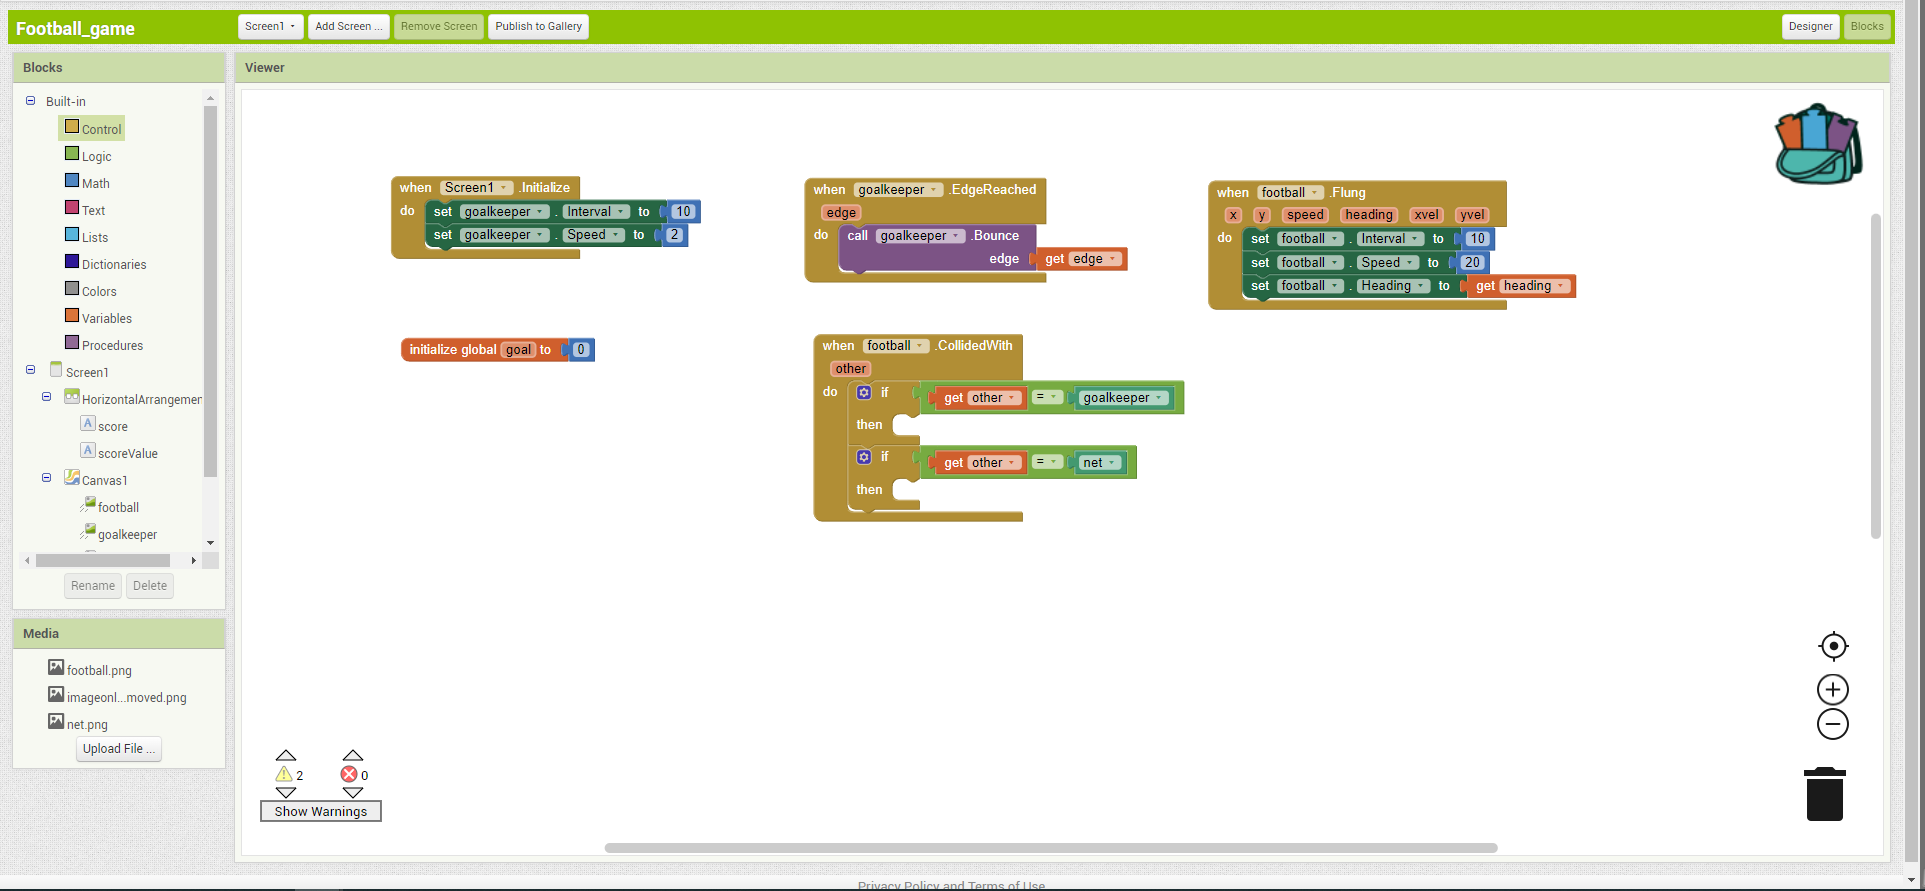
\includegraphics[width=1.0\linewidth,height=0.5\linewidth]{fig110011.png}
  \caption{Добавяне на проверките}
\label{fig110011}
\end{figure}

Когато топката докосне вратаря играта трябва да приключи. Казано с езика на инструкциите трябва да се променят някои от свойствата на топката и да се покаже съобщение, че играта е приключила. Първото свойство на топката, което трябва да се промени е това Enabled да е със стойност false. Това означава, че няма да се движи. Следва да се промени позицията ѝ. Стойностите за координатите са x=120, y=320 и z=1. Свойството Speed трябва да се промени да бъде 0.

За да се появи диалогово съобщение се добавя инструкция от елемента Notifier1, която е ShowMessageDialog. Тя трябва да има следните полета - message="Game over", title, което се състои от score.Text и scoreValue.Text и поседното е buttonText="Restart game". Когато приключи играта трябва да се върнат първоначалните стойности на променливата, която е 0, на текстовото поле за scoreValue, което също е 0. Не трябва да се забравя да се промени и стойнсотта на топката Enabled да бъде true, за да може отново да се движи топката.

\begin{figure}[H]
  \centering
  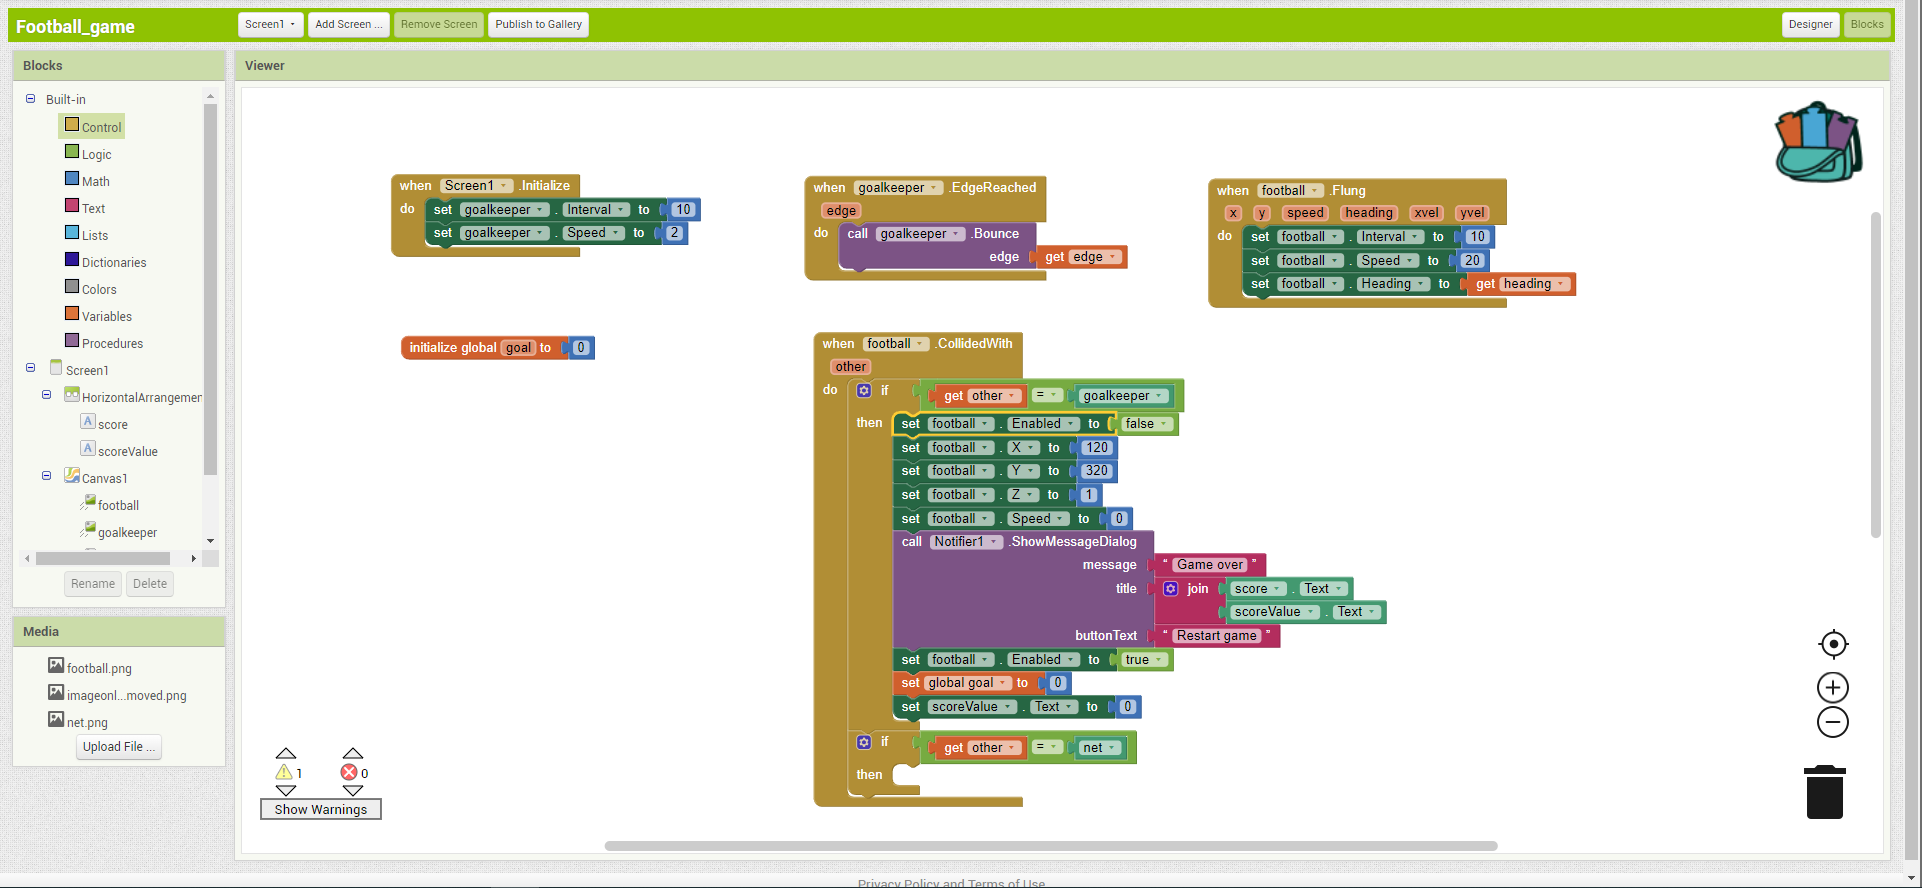
\includegraphics[width=1.0\linewidth,height=0.5\linewidth]{fig110012.png}
  \caption{Когато топката докосне вратаря}
\label{fig110012}
\end{figure}

Когато топката докосне мрежата, инструкциите са долу горе аналогични. Първо трябва да се промени позицията на топката. Разликата е в това, че трябва да се увеличи променливата и да се покаже новия резултат.

\begin{figure}[H]
  \centering
  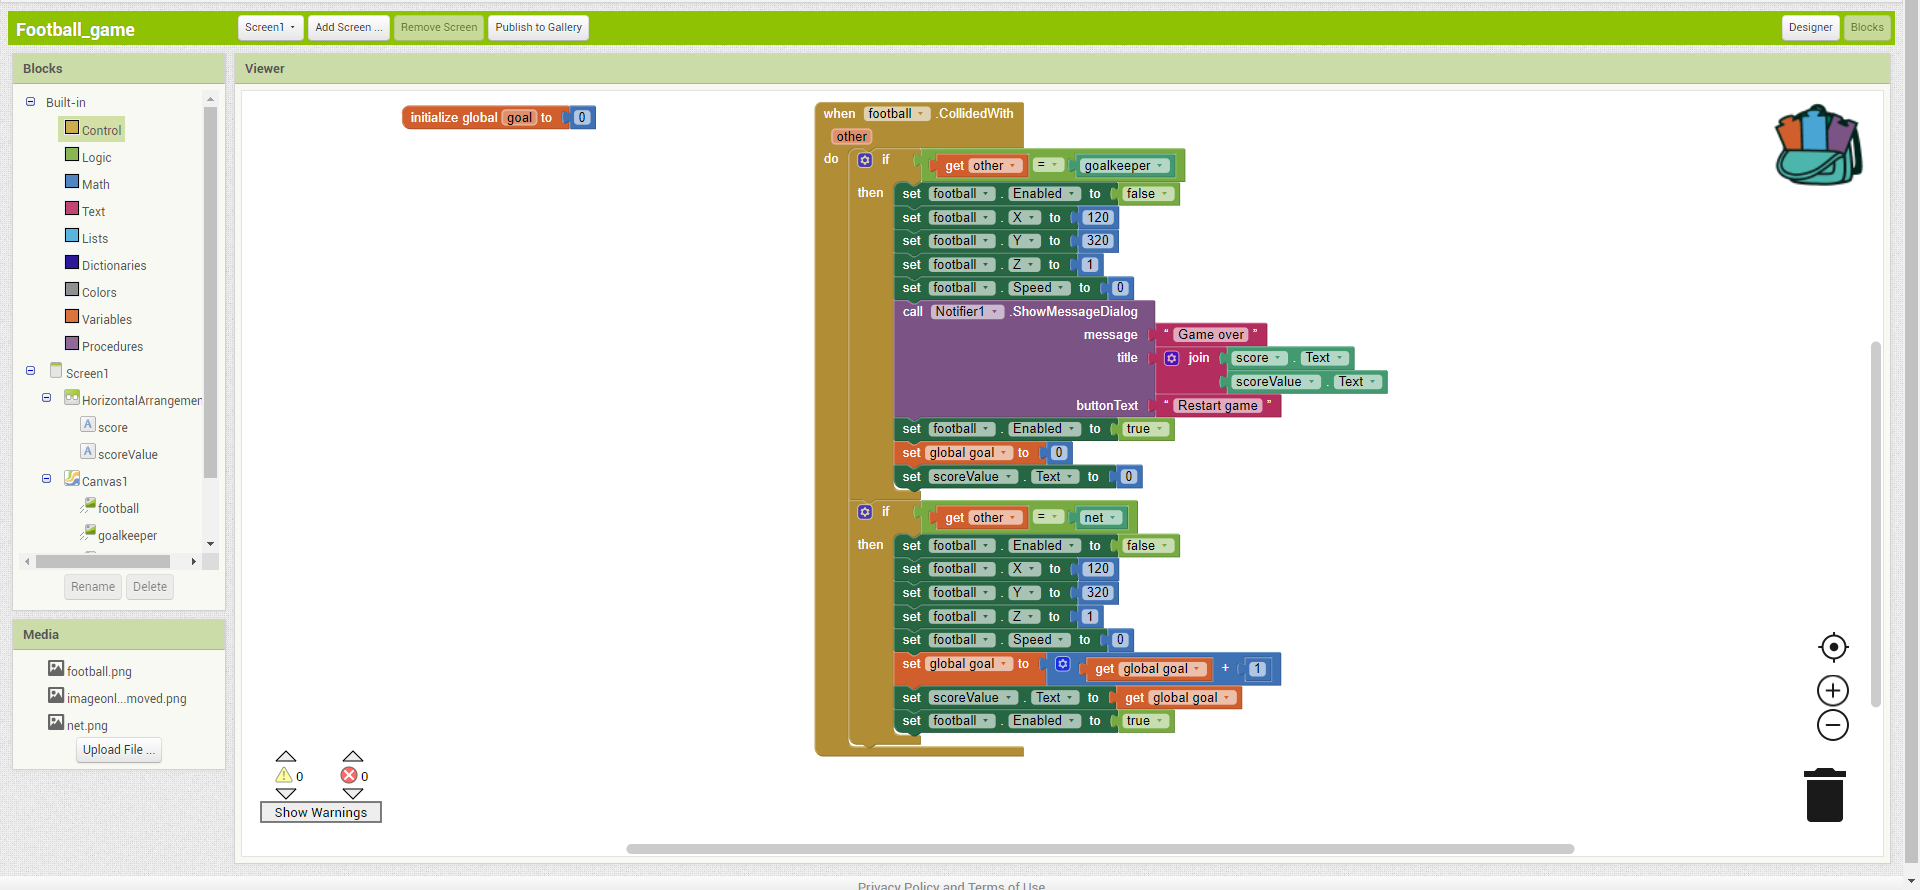
\includegraphics[width=1.0\linewidth,height=0.5\linewidth]{fig110013.png}
  \caption{Когато топката докосне мрежата}
\label{fig110013}
\end{figure}

Играта е готова. Може да направите състезание с приятелите си, за да видите кой е по- добър във вкарването на голове.